\chapter{Integration Design and Architecture}
\label{cha:integration_design_and_architecture}

This chapter presents the design of the solution developed in this work to connect Legion clients to Antidote data storage. We start by briefly presenting Antidote and Legion, focusing on the mechanisms necessary for integrating both systems. After this introduction, we presents an overview of the proposed design and the interaction between Legion and Antidote.

\section{Overview of used systems}
\label{sec:system_introduction}
In order to design an integration between Legion and Antidote, it is imperative that we understand how both systems work, so we can take advantage of their internal mechanisms to our advantage. Next follows a brief presentation of the mentioned systems, as well as some important working details.

\subsection{Legion}
\label{sec:legion_intro}
A large number of web application are built around direct interactions among clients, such as collaborative applications, social networks and multi-user games. These applications manage a set of shared objects, with each user reading and writing to a subset of these objects. These kind of applications are usually implemented using a centralized infrastructure that maintains the shared state and mediates all interactions among users. This approach has some drawbacks, such as the servers becoming a scalability bottleneck, the service interrupt when the servers are unavailable and the latency of nearby users being unnecessarily high.\par
	One alternative to this model, is to rely on direct communication between users. In a not so far past, such an alternative would be troublesome when combining peer-to-peer and Web applications. Due to the lack of supporting mechanisms for this, it was often needed browser extensions or plugins to implement such a scenario.\par
	With the recent development of tools such as WebRTC, that enables direct communication between browsers and connectivity utilities such as STUN and TURN that can overcome the trouble of connecting users between NATs and firewalls, a new set of peer-to-peer web applications started to be developed.\par
	Legion is a framework that exploits these new features for enriching web applications with direct data replication between browsers. Each client maintains a local data storage with replicas of a subset of application shared objects. Legion uses an eventual consistency model, where each client can modify its local objects without coordination, this allows updates to be performed concurrently on different replicas while modifications are propagated asynchronously. To guarantee that all replicas converge to the same correct state after updates have been applied on different replicas, Legion relies of CRDTs as its internal data structure. To support these interactions in a peer-to-peer manner, clients form overlay networks to propagate objects and updates among them. In each overlay network, a few clients act as synchronization point of a possible centralized component. These clients have an objects server component that is design to support extensions with legacy storage systems to act as centralized persistent storage. This component has a view of the Legion group objects, which can be used as a replication point of the system state to a centralized storage system. The external system will use Legion's primitives, available in the communication API, in order to propagate updates back and forward. These updates are sent in a point-to-multipoint fashion, by delegating the afford of propagating the updates to all the legion clients in the group to a node which carries the objects server. Overall, image \ref{legion_architecture} illustrates how an external centralized storage system can interact with Legion, as well as Legion's architecture.
	
\begin{figure}[H]
\centering
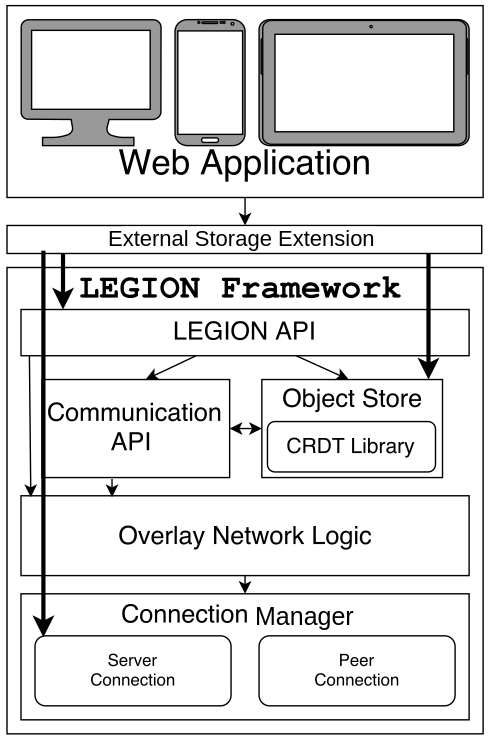
\includegraphics[scale=0.3]{files/legionArchitecture.png}
\caption{Legion Architecture}
\label{legion_architecture}
\end{figure}

\subsection{Antidote}
\label{sec:antidote_intro}
Traditional databases provide strong guarantees but are slow and unavailable under failures and network partition. Hence, they are not suitable for geo-replication. The alternatives are NoSQL-style databases which are fast and available even under network partition. They provide a low-level key-value interface and expose data inconsistencies due to asynchronous communication among the servers. It takes significant effort and expertise from programmers to deal with these inconsistencies and develop correct applications on top of these databases. Antidote provides features that aid programmers to write correct applications, while having the same performance and horizontal scalability as NoSQL, from a single machine to geo-replicated deployments, with the added guarantees of Causal Highly-Available Transactions, and provable absence of data corruption due to concurrency.\par
	Internally, Antidote uses CRDTs as data structures. To modify these, one can make use of interactive transaction composed by three steps: start, update/read and finally commit. Transactions can receive a timestamp to force the read/update to be executed at a certain system snapshot. Another import API method is the ability to request the executed operations log since a certain timestamp. Antidote clients can use this API via the distributed Erlang interface that can only be used by Erlang clients, or the protocol buffer interface, which is language independent. Antidote can work in cluster mode, with several nodes in the same cluster that replicate data using the saved logs, or in inter-dc mode by simply replicating data in a FIFO (First in first out) operation order. The system architecture can be visualized in image \ref{antidote_architecture}.

\begin{figure}[H]
\centering
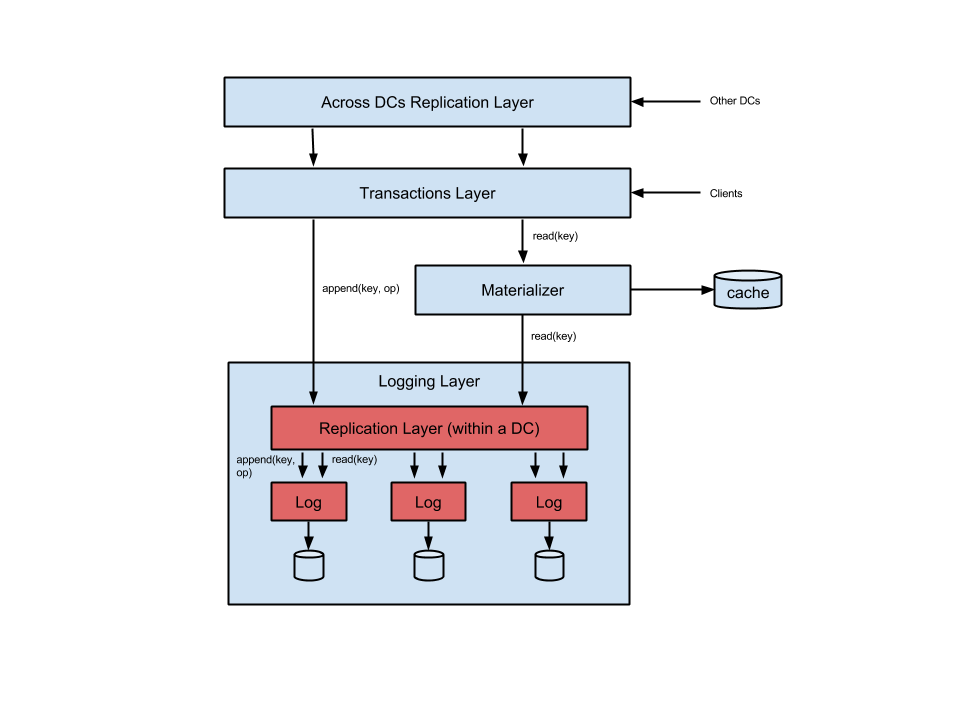
\includegraphics[scale=0.4]{files/antidoteArchitecture.png}
\caption{Antidote Architecture}
\label{antidote_architecture}
\end{figure}

\section{Architecture Overview}
\label{sec:architecture_overview}
Legion includes a mechanism to allow the integration with other external storage systems. This mechanism consists in a module that implements a pre-defined interface.\par
	Figure \ref{architecture} shows the architecture of our approach to integrate Legion with Antidote. The following components are included in the architecture.
	
\begin{figure}[h]
\centering
\includegraphics[scale=0.5]{files/architecture.png}
\caption{Integration Architecture}
\label{architecture}
\end{figure}

\par
	The integration of Legion and Antidote can be depicted into the following components:
\begin{description}

\item[Antidote] \hfill \\
The storage system to be integrated with Legion. Antidote will act as a persistent, stable, client-server model storage system. It will be synchronized with Legion, so both will have the entire set of updated objects in the system. An Antidote node can have it's data updated directly from an antidote client, or from an update that was propagated from Legion nodes.\par
Besides that, Antidote will also keep meta-data related to the system synchronization, such as propagated operations identifiers and elements' unique tokens.

\item[Antidote Client] \hfill \\
This component is one of the entry points of information into the system. An Antidote client can manipulate the system's data set by making calls to modify the state of Antidote's objects.\par
	This client is written in javascript and it uses the integration proxy in order to make read and write requests because a direct request can not be made from a browser due to cross-origin security. These requests have a flag to distinguish them from the objects server requests.


\item[Legion Node] \hfill \\
This component is a Legion instance in the system. It acts as an entry point of information to the system and it also as the responsibility to keep it self and the other Legion nodes updated and synchronized.


\item[Legion's Objects Server] \hfill \\
This component keeps a global view of what is happening in the Legion network. There can be one or more objects servers in the system, and Legion's synchronization events will pass through at least one of these. In the objects server also resides the logic for the synchronization between Antidote and Legion. This is done by watching for object update events and then propagating them.\par
This component is written in NodeJS and it uses the integration proxy for the communication with Antidote, by making read and write calls.

\item[Integration Proxy] \hfill \\
This component is needed to establish communication with Antidote. There can be one or more integration proxies in the system. It takes advantage of Antidote's protocol buffer interface to make read and write calls.\par
The proxy can receive requests from either a Antidote client or a Legion's object server synchronization method. The request is parsed and a call is sent to Antidote. When the answer from antidote is received, it is redirected to who made the request. This component is written in NodeJS.

\item[ZooKeeper Service] \hfill \\
ZooKeeper is used in the system as a service in order to guarantee mutual exclusion of meta-data updates from different sources. It receives locking requests from all the integration proxies and keeps information of the locking status of each system object.

\end{description}

\section{Integration challenges}
\label{sec:integration_challenges}
When integrating both systems, there were some challenges there we had to tackle and overcome. The main effort in this integration is the synchronization, initially we tried to follow the path of merging CRDTs directly, but as explained before, Antidote didn't offer the needed mechanisms to make this happen. The synchronization was then changed to be about operation propagation. This brings some questions regarding the needed metadata and the operations order. For the first topic, it was needed to keep operation identifiers, as well as CRDT tokens, both stored in Antidote. Having metadata modified from different sources heeds concerns about data corruption. We need to assure that updates to this structure is done safely. About the second topic, applying past operations in another systems requires that the updates are executed at a certain system snapshot.\par
	The solution of these challenges are depicted next in sections \ref{sec:legion_to_antidote_flow} and \ref{sec:antidote_to_legion_flow}, by explaining step by step how the data is propagated between systems, keeping the system's objects synchronized along with the related metadata.

\section{Legion to Antidote flow}
\label{sec:legion_to_antidote_flow}
This section explains the process of propagating an update issued by a Legion node into Antidote. Algorithm \ref{legion_to_antidote_algorithm} depicts the sequence of events.\par
	In order to send the updates from Legion to Antidote we must first detect these updates. To do so, we opted for an event driven model, by relying on Legion's objects server, since every update issued by a Legion node will end up in at least one of the objects servers.\par
	Once the event is detected in the objects server, the incoming message is filtered based on the event type. If the event contained in the message is indeed an update, that objects server will issue one or more update requests to the integration proxy. Once a request reaches the integration proxy, this one will decouple the request into the the actual update data and meta-data. These two are then sent to Antidote as write requests. Besides writing the data into Antidote, the Integration proxy certifies that the operation has not been executed already, since there can be more than one objects server to issue the request. This is done by checking the meta-data stored in Antidote.\par
	Once the update reaches Antidote successfully, the integration proxy returns to the objects server.
	
\begin{algorithm}
\caption{Legion to Antidote flow}
\label{legion_to_antidote_algorithm}
\begin{algorithmic}[1]
\algblock{Upon}{End}
\Upon { $event$:}
  \If {$event.type$ = $update$}
    \State {objectsServer.apply($update$)}
    \State {$metaData$ $\gets$ parse($update$)}
    \State {$doneOperation$ $\gets$ antidote.read($doneOperations$)}
    \If {!($update.id$ in $doneOperations$)}
      \State {zooKeeper.lock($metadata.objectId$)}
      \State {antidote.write($metadata$)}
      \State {zooKeeper.unlock($metadata.objectId$)}
      \State {antidote.write($update.operations, lastSeenTimestamp$)}
      \State {return}
    \EndIf
  \EndIf
\End
\end{algorithmic}
\end{algorithm}

\section{Antidote to Legion flow}
\label{sec:antidote_to_legion_flow}
This section explains the process of propagating an update issued by an Antidote client into Legion. Algorithm \ref{antidote_to_legion_algorithm} shows this process step by step.\par
	When an Antidote client issues an update, it is firstly sent to the integration Proxy. This one receives the request and sends them to Antidote. This is due to the cross-origin security. The integration proxy returns to the client when the update is successful.\par
	The next step is to send this update to every Legion node. This can be done by sending the update to the objects servers, which will then propagate the message to every node.\par
	At this point there are two methods of sending the update to the objects server. It can be done with a public/subscribe system that fires an event each time an Antidote object is updated, or having Legion's objects servers to probe periodically for new updates on Antidote. The first option would definitely be more performant, because scanning Antidote periodically for updates would have some overhead. With this in mind we talked to the development team in order to know the best way to to this. One alternative was to use Antidote's internal updates propagation mechanism to also fire an event to the exterior, but this solution had two major problems. The update propagation mechanism would not handle lost messages, this would have to be handled by us, and to exposed such internal mechanism to the outside would go against the Antidote's design path. With this, we concluded that we should proceed to the second option.\par
	In order to periodically check for updates in Antidote, we used the system log to get the operations executed since a certain timestamp.\par
	Legion's objects servers will periodically make a request to the integration proxy, in order to check the operations executed in Antidote since the last seen timestamp. The proxy relays the request to antidote and returns the result. If there are no new updates, then the objects server only updates it's last seen timestamp. If there are new updates that were not propagated to legion, the objects server executes the operation locally, and then propagates it to every Legion node.
	
\begin{algorithm}
\caption{Antidote to Legion flow}
\label{antidote_to_legion_algorithm}
\begin{algorithmic}[1]
  \algblock{Every}{End}
  \Every { 2 seconds:}
  \State {$logOperations$ $\gets$ antidote.get($logOperations$, $lastSeenTimeStamp$)}
    \ForEach {$operation \in logOperations$}
      \If {!($operation.id$ in objectsServer.$doneOperations$)}
        \State {$metadata$ $\gets$ parse($operation$)}
        \State {zooKeeper.lock($metadata.objectId$)}
        \State {antidote.write($metadata$)}
        \State {zooKeeper.unlock($metadata.objectId$)}
        \State {objectsServer.Apply($operation$)}
        \State {legion.Propagate($operation$)}
      \EndIf
    \EndFor
    \State {objectsServer.update($lastSeenTimestamp$)}
    \State {return}
  \End
\end{algorithmic}
\end{algorithm}